\section{Introduction}
\label{sec:intro}
% Intro structure:
% 1. What is the problem?
% 2. Why is it important?
% 3. Why is the problem hard? What makes it challenging?
% 4. How far has existing work come? Cite a few papers. What is the next frontier?
% 5. Why hasn’t the problem been solved? What is the stumbling block?
% 6. What does our paper contribute?
% 7. What is the key idea? What is the magic trick? What is the new insight or technique that enables us to advance the frontier?
% 8. What do the experiments say?
\begin{figure}[t!]
    \centering
    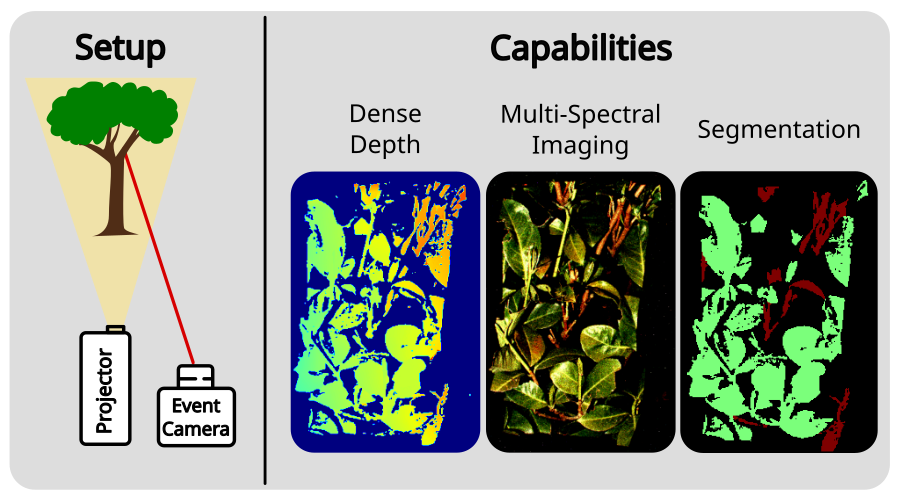
\includegraphics[width=.8 \textwidth]{resources/images/overview.png}
    \caption{Method description}
    \label{fig:method_overview}
\end{figure}

% 1. What is the problem?
Limitations of multispectral cameras for material classification and identification, specifically regarding spatial and temporal resolution, spectral resolution.

% 2. Why is it important?
It is important to overcome these limitations because accurate material classification and identification are crucial for various applications, including industrial sorting, automated manufacturing, product defect detection, and safe robot navigation.

% 3. Why is the problem hard? What makes it challenging?
The problem is challenging because existing multispectral cameras sacrifice spatial and temporal resolution for spectral resolution. 
Snapshot methods sacrifice spectral resolution for spatial resolution, while point or line-scanning spectrometers sacrifice temporal and spatial resolution for spectral resolution. 
Additionally, the lack of depth information further hampers robust material identification.

% 4. How far has existing work come? Cite a few papers. What is the next frontier?
Existing work has focused on improving the capabilities of multispectral cameras. 
The next frontier lies in developing a system that combines multispectral sensing, depth reconstruction, and event-based imaging to address the shortcomings of traditional approaches.

% 5. Why hasn’t the problem been solved? What is the stumbling block?
The problem hasn't been solved because existing methods have limitations in terms of resolution, spectral fidelity, and depth information. 
Traditional multispectral cameras struggle to capture fine spatial details and exhibit limited temporal resolution, making them less effective for dynamic scenes. 
The absence of depth information further limits their robustness and accuracy in material classification.

% 6. What does our paper contribute?
Our paper contributes by proposing an event-camera based system for multispectral sensing and depth reconstruction. 
This system leverages a point-scanning approach with a fast scanner, enabling high temporal resolution, rapid scanning, and enhanced robustness to lighting variations. 
The combination of point scanning and event cameras allows for more accurate depth computation compared to conventional approaches.

% 7. What is the key idea? What is the magic trick? What is the new insight or technique that enables us to advance the frontier?
The key idea is to utilize an event-based multispectral and depth sensing system to overcome the limitations of traditional multispectral cameras. 
By combining event cameras with point scanning, we achieve high temporal resolution and accurate depth computation. 
This approach offers advantages in material classification applications, paving the way for future advancements in the field.

% 8. What do the experiments say?
The experiments conducted in this paper demonstrate the potential of the proposed event-based multispectral and depth sensing system. 
The results highlight its efficacy in material classification applications, showcasing its advantages over traditional multispectral or depth imaging sensors. 
These findings provide a promising direction for further advancements in the field.

Our contributions can be summarized as follows:
\begin{itemize}
    \item We extend the proposed event-based structured light setup for intensity reconstruction.
    Event cameras pose a challenge as they only measure logarithmic intensity changes. 
    Estimating the intensity is not trivial as it requires knowledge of the sensor contrast threshold, which is not available. 
    To overcome this obstacle, we propose a methodology that involves estimating the contrast threshold and subsequently predicting the absolute intensity.
\end{itemize}